\section{Ejercicio 5: Comparación}

  % \begin{figure}[ht]
  %   \begin{center}
  %     \includegraphics[width=0.5\columnwidth]{imagenes/pacman.png}
  %     \caption{Perdidos y con poca fuerza}
  %   \end{center}
  % \end{figure}

    % 1. Describir detalladamente el problema a resolver dando ejemplos del mismo y sus soluciones.
    \subsection{Hipótesis}
        Para realizar un análisis exhaustivo y poder realizar conclusiones generales sobre las distintas implementaciones de nuestro problema, se pidió por último hacer una experimentacion acorde para poder compararlas, utilizando donde sea posible las mejores configuraciones halladas (particularmente para los ejercicios 3 y 4).
        Las instancias que creamos fueron pensadas para intentar obtener la mayor variedad de resultados entre cada experimento, pero también se usaron nuevas instancias generadas de manera aleatoria pero intentando tener la mayor probabilidad de que cada una de esas instancias tenga solución.

        Para la búsqueda local se utilizó el vecindario A, mientras que para Grasp se usó de la siguiente forma: Vecindario A, RCL 3 y criterio de parada 1, con limite 100.

        Teniendo en cuenta la experimentación realizada a lo largo de este trabajo, esperábamos que la metaheruística tenga mejores resultados que la heurística greedy y la búsqueda local, pero que no haya mucha diferencia temporal entre ellas incluso para instancias grandes y a pesar de la cota de complejidad propuesta para el ejercicio 3.

    \subsection{Experimento 1}
        En este experimento se utilizaron instancias que tenían una solución "única", es decir, era necesario pasar por todas las pokeparadas para poder conquistar todos los gimnasios. La que podía variar es el órden en que se recorren las estaciones para obtener la solución, dejando lugar a que el algoritmo de herústica greedy pueda fallar. Las ubicaciones de las estaciones estan puestas de manera secuencial $gimnasio-pokeparada-gimnasio-pokeparada$ en las posiciones $(i,i)$ de un plano. Así, el camíno óptimo (y por lo tanto solución correcta) sería comenzar desde la primera pokeparada (0,0) y desde ahí alejarse en diagonal, para obtener las pociones necesarias para el siguiente gimnasio en cada iteración.
        Para intentar obtener una variación de este mismo tipo de instancia, cambiamos la ubicación de la pokeparada desde la cual se debería comenzar a la posición más lejana del (0,0) y en cada iteración hay que acercarse en 1 al (0,0). 

        Para la primera versión de estas instancias, los resultados obtenidos en cuanto a tiempo de corrida de cada algoritmo se graficaron de la siguiente manera:

        \blindtext

        \begin{figure}[H]
        \minipage{0.5\textwidth}
          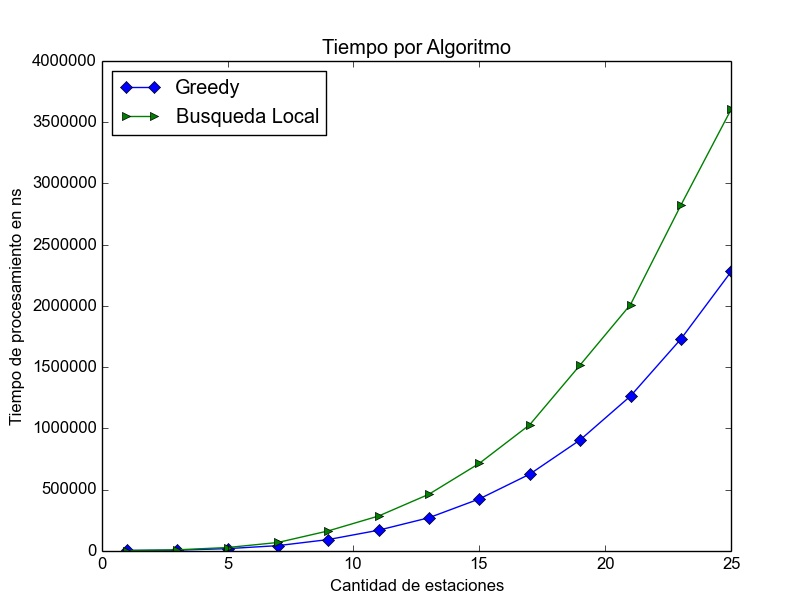
\includegraphics[width=\linewidth]{imagenes/exp1a_ej5_tiempo_sin_BT.jpeg}
          \caption{Sin BT ni GRASP}
        \endminipage\hfill
        \minipage{0.5\textwidth}%
          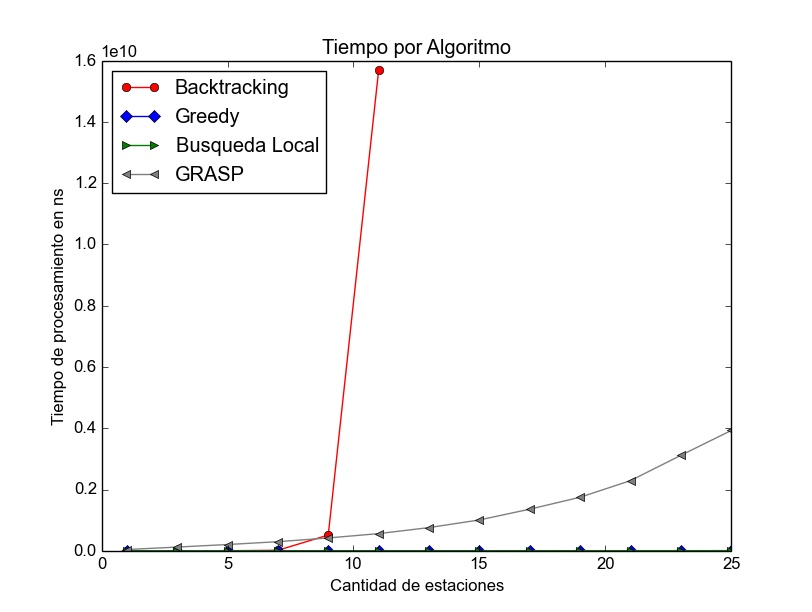
\includegraphics[width=\linewidth]{imagenes/exp1a_ej5_tiempo_con_BT.jpeg}
          \caption{Con BT}
        \endminipage
        \end{figure}

        \blindtext

        La razón por la que lo separamos en dos graficos es porque las instancias ejecutadas con Backtracking, como se puede apreciar en el gráfico, hacían que las líneas que representan a los otros algoritmos no puedan apreciarse en el mismo. Observando el eje $y$ de cada grafico podemos notar la gran diferencia que hay de tiempo en instancias de tan solo 8 estaciones. Los otros 3 algoritmos se corrieron con hasta 25 estaciones y ninguno lograba alcanzar un tiempo similar.

        Podemos notar también que, con sentido, el algoritmo que solo realiza una heurística greedy es el que menos tiempo toma en ejecutar. En las próximas figuras hacemos una comparacion de qué tan bueno es que tome tanta diferencia de tiempo.

        \begin{figure}[H]
            \begin{center}
              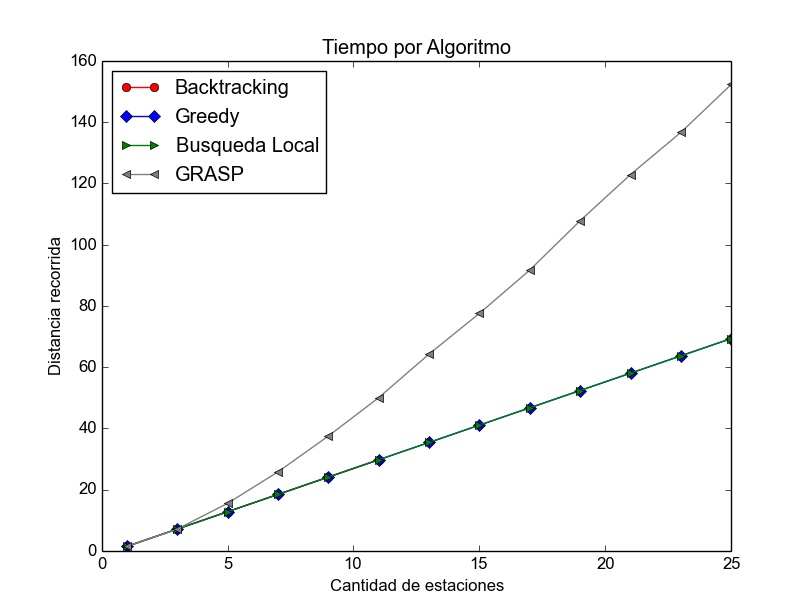
\includegraphics[width=0.7\columnwidth]{imagenes/exp1a_ej5_correctitud_solucion.jpeg}
              \caption{}
            \end{center}
        \end{figure}

        Tal como esperabamos, en este primer tipo de instancias, los resultados fueron exactamente los mismos para todos los algoritmos en cuanto a distancia recorrida. Lo que podemos concluir de esta primera parte es que para las instancias que tienen cierto "orden" (es decir, se puede empezar en un punto e ir en linea recta sin tener que pasarse a todas las otras estaciones), el mejor algoritmo será el de la heurística greedy, ya que de todos es el que menos tiempo toma y aún así da una solucion acertada.

        Para el segundo tipo de instancias, el resultado de los tiempos fueron los siguientes:

        \begin{figure}[H]
        \minipage{0.5\textwidth}
          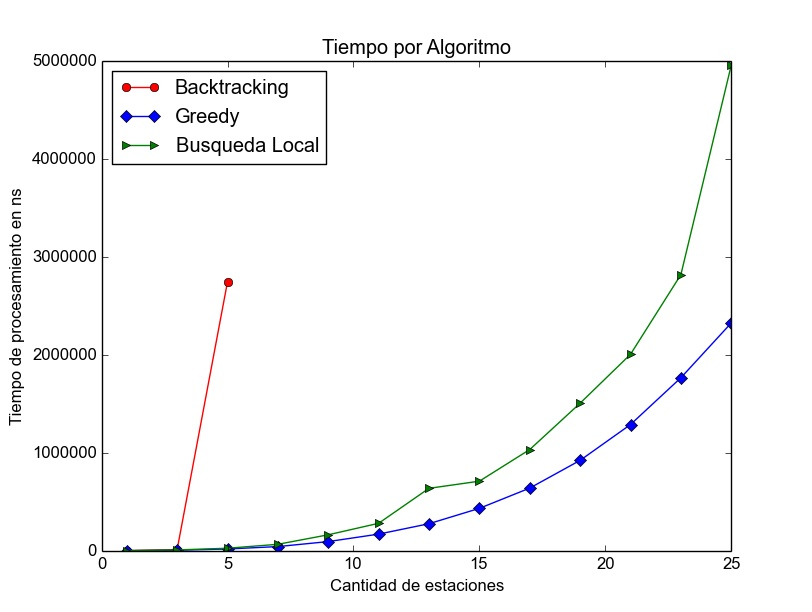
\includegraphics[width=\linewidth]{imagenes/exp1b_ej5_tiempo_con_BT.jpeg}
          \caption{Sin GRASP}
        \endminipage\hfill
        \minipage{0.5\textwidth}%
          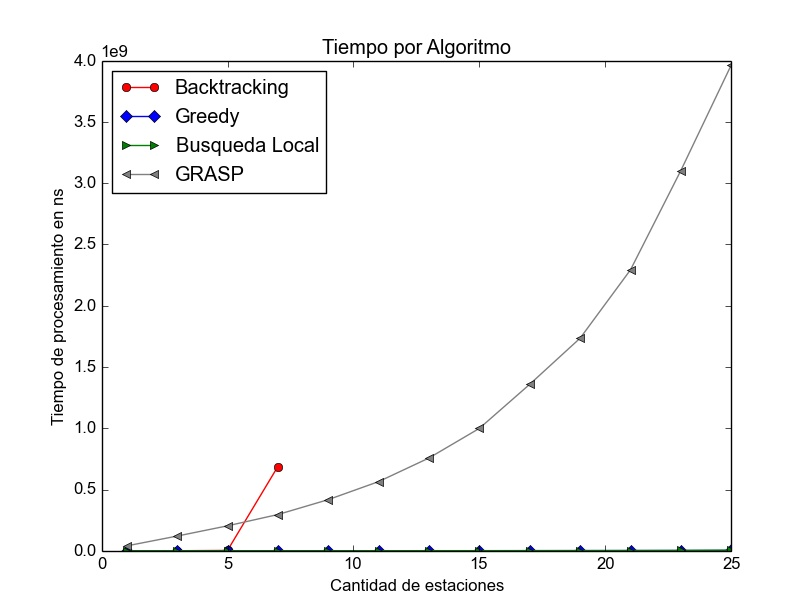
\includegraphics[width=\linewidth]{imagenes/exp1b_ej5_tiempo_con_BT_con_MT.jpeg}
          \caption{Con GRASP}
        \endminipage
        \end{figure}

        En cuanto a soluciones obtenidas, los graficos fueron los siguientes:

        \begin{figure}[H]
            \begin{center}
              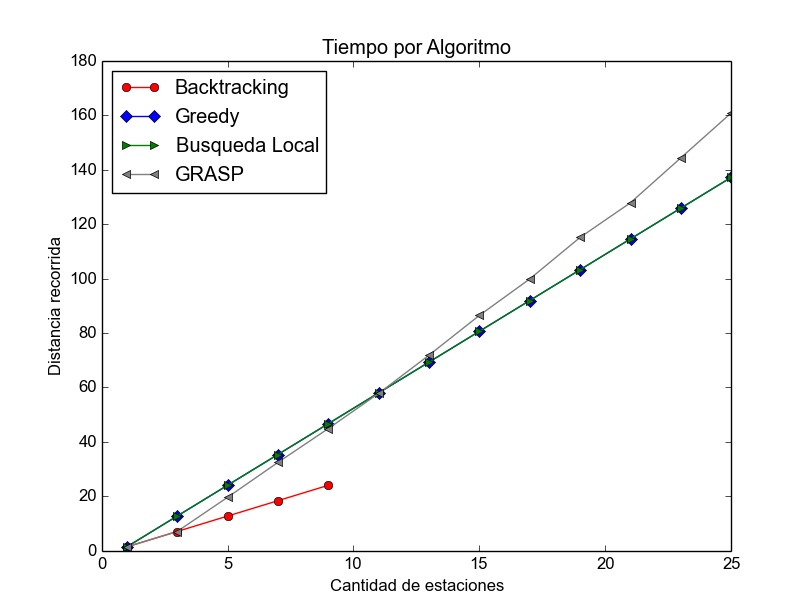
\includegraphics[width=0.7\columnwidth]{imagenes/exp1b_ej5_correctitud_solucion.jpeg}
              \caption{}
            \end{center}
        \end{figure}

    \subsection{Experimento 2}
        Para este segundo experimento se setearon más pokeparadas que gimnasios y se ubicaron de manera tal que en un plano las posiciones formarían un pico (por ejemplo, $g$(1,1), $g$(1,5), $p$(2,2), $p$(2,4), $p$(3,3)). Los gimnasios requerían pasar al menos por una pokeparada excepto el gimnasio más cercano al eje $x$ pero que de los dos más cercanos es el más lejano al (0,0), el cual se seteó con 0 pociones (y todos los demás con 1). Para estas instancias, siempre hubo 1 pokeparada más que gimnasios.

        Un ejemplo de estas instancias es la siguiente: 

\begin{codesnippet}
      \begin{verbatim}
      6 7 100
      1 1 1
      1 13 0
      3 3 1
      3 11 1
      5 5 1
      5 9 1
      2 2
      2 12
      4 4
      4 10
      6 6
      6 8
      7 7
      \end{verbatim}
\end{codesnippet}

      Los resultados obtenidos fueron:


      \begin{figure}[H]
        \minipage{0.5\textwidth}
          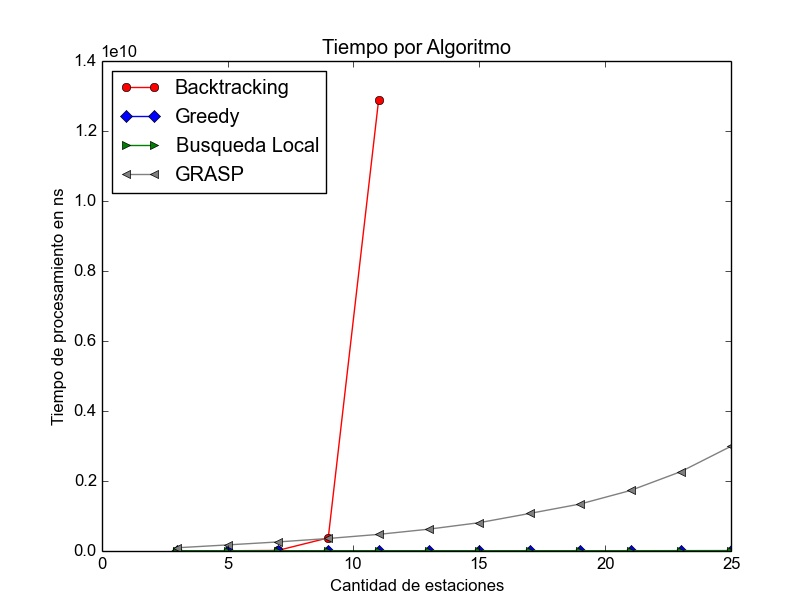
\includegraphics[width=\linewidth]{imagenes/exp2_ej5_tiempo_con_BT.jpeg}
          \caption{Con BT y GRASP}
        \endminipage\hfill
        \minipage{0.5\textwidth}%
          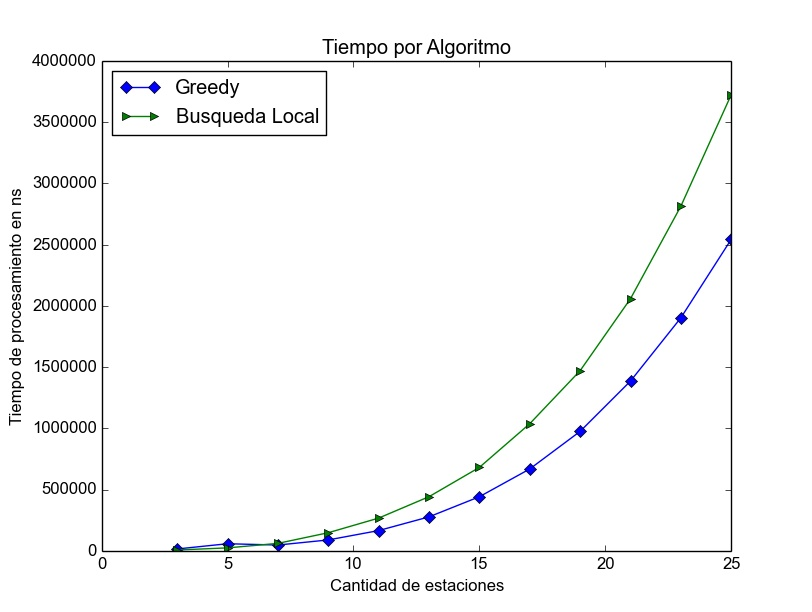
\includegraphics[width=\linewidth]{imagenes/exp2_ej5_tiempo_sin_BT_ni_GRASP.jpeg}
          \caption{Sin BT ni GRASP}
        \endminipage
        \end{figure}

        En cuanto a tiempos de ejecicion.
        En cuanto a calidad de soluciones, obtuvimos:


        \begin{figure}[H]
            \begin{center}
              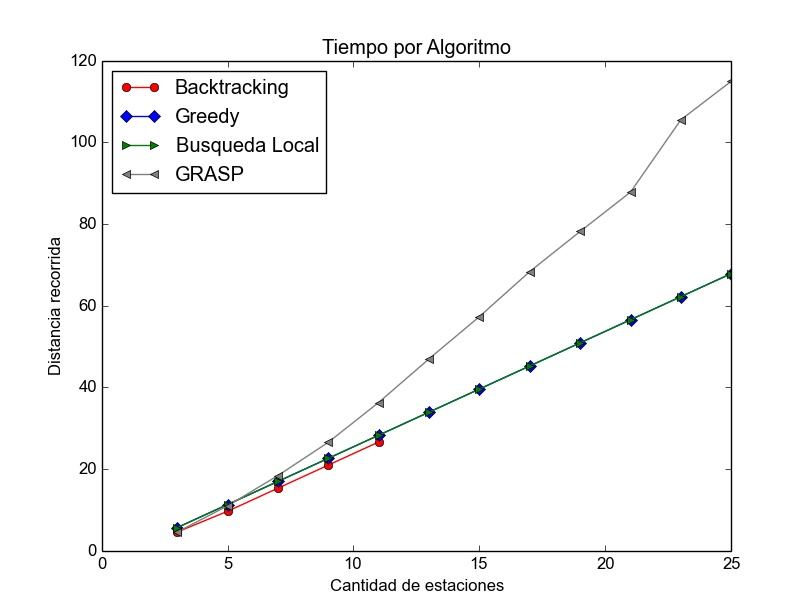
\includegraphics[width=0.7\columnwidth]{imagenes/exp2_ej5_correctitud_solucion.jpeg}
              \caption{}
            \end{center}
        \end{figure}
      